\documentclass[]{beamer}



\usepackage{amssymb}
\usepackage{graphicx}
\usepackage{subfigure}
\usepackage{framed}
\usepackage{subfiles}
\usepackage{newlfont}
\usepackage{amsmath,amsthm,amsfonts}
%\usepackage{beamerthemesplit}
\usepackage{pgf,pgfarrows,pgfnodes,pgfautomata,pgfheaps,pgfshade}
\usepackage{mathptmx}  % Font Family
\usepackage{helvet}   % Font Family
\usepackage{color}

\begin{document}
%% Chapter 4
%% \chapter{Tools of Support to MSQC}

\section{4.1 Tools of Support to MSQC}
\begin{frame}[fragile]
\begin{itemize}
	\item As a general rule, normality and independence of the data is required in Statistical Process Control and the multivariate extensions are not the exception. 
	
	\item In a multivariate control chart with the use of rational subgroups according to the central limits theorem certain grade of normality is achieved. But in alternatives called charts for individuals, this rule is not satisfied. The same occurs in capability indices that rarely are computed using subgroups.
	
	\item Many authors have proposed nonparametric alternatives to deal with the
	departures of normality and techniques based on PCA as the studied in Sections 2.10 and 3.6 which are robust to the lack of normality.
	\item However, nowadays it results quite unproblematic to test multivariate normality and randomness. In this chapter we introduce a wide range of tools to fulfill these requirements.
\end{itemize}
\end{frame}


\section{4.1.1 Graphical Methods}
\begin{frame}
The first section of this chapter will examine two graphical techniques: histogram
and Q-Q plot that facilitate the assumption of normality.
Histogram is a graphical technique that allows a visual summary of the data. It
provides information about the center, the spread, the skewness, and the existence
of outliers. (NIST / SEMATECH e-Handbook of Statistical Methods).
\end{frame}
%=============================================%
\begin{frame}[fragile]
A visual inspection of a histogram permits to establish an initial hypothesis of
the distribution; in this case a bell-shaped is desired.
Although histograms are basically used in univariate scenarios, univariate
normality per se does not imply multivariate normality; if a departure from normality
is founded in individual variables, this has a negative effect in the
multinormality.
\end{frame}
%E. Santos-Ferna´ndez, Multivariate Statistical Quality Control Using R,
%SpringerBriefs in Statistics 14, DOI 10.1007/978-1-4614-5453-3_4,
%# Springer Science+Business Media New York 2012
%87
%-------------------------------------------------------------------------------------%
\subsubsection{Example 4.1}
\begin{frame}
In this example we will illustrate the use of histogram in a multivariate context. For
that, return to the bimetal dataset introduced in Sect. 2.6.
To put multiple figures in one graph device the parameter mfrow can be used by
specifying \texttt{mfrow = c(n,m)} being n the number of figures by row and m by columns.

As for each quality characteristic a histogram is desired—a simple loop is used.
\end{frame}
%=============================================%
\begin{frame}[fragile]
\begin{verbatim}
> par(mfrow = c(3,2))
> for( i in 1 : ncol(bimetal1) ){
> x <- bimetal1[,i]
> mean<-mean(bimetal1[,i])
> sd<-sd(bimetal1[,i])
> hist(x, prob = TRUE, main = paste( "Histogram for ", colnames(bimetal1)[i] ),xlab = "")
> Finally, adding the normal curve
> points(curve(dnorm(x, mean = mean, sd = sd), add = TRUE),type = "l")}
\end{verbatim}
\end{frame}
%=============================================%
\begin{frame}[fragile]
From this chart we can appreciate that most of the classes are located in the center,
no significant skewness is revealed, no long tails are presented, and no considerable
outliers are detected. The form of the classes does not differ drastically to the normal
shape. Finally, there is no visual evidence to reject the univariate normality hypothesis.
\end{frame}
%=============================================%
\begin{frame}[fragile]
This visual inspection can be complemented with the quantile-quantile plot, or simply Q-Q plot. The Q-Q plot is a graphical tool for comparing a two dataset or a dataset with a
theoretical distribution. The most common use is to plot the quantiles against a Histogram for Deflection Density
\end{frame}
%=============================================%
\begin{frame}[fragile]
\begin{figure}
\centering
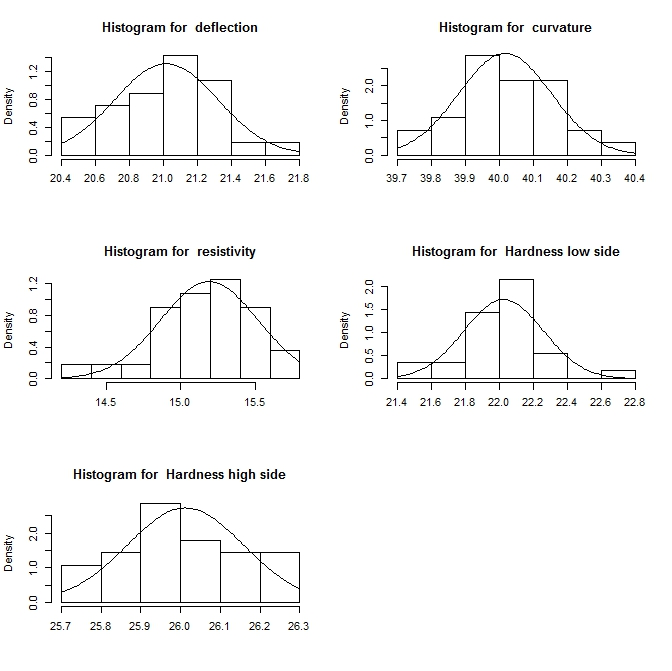
\includegraphics[width=0.7\linewidth]{MSQC-bimetal1hist}
\caption{}
\label{fig:MSQC-bimetal1hist}
\end{figure}
\end{frame}
%=============================================%
\begin{frame}[fragile]

Fig. 4.1 Histogram of the individual variables in the bimetal1 dataset
%% 88 4 Tools of Support to MSQC
%-------------------------------------------------------------------------------------%


%-----------------------------------------------------------------------------------%
reference line from a normal distribution. When the points fall approximately over
the line there is evidence that both come from an identical distribution.
The performing of a Q-Q plot in R is done through the qqnorm function.
\end{frame}
%=============================================%
\begin{frame}[fragile]
\frametitle{Example 4.2}

To construct a Q-Q for each variable from bimetal1 dataset:
\begin{verbatim}
> par(mfrow = c(3,2))
> for( i in 1 : ncol(bimetal1) ){
> qqnorm(bimetal1[,i], main = paste( "Q-Q plot for ", colnames(bimetal1)[i] ) )
> qqline(bimetal1[,i])
> }
\end{verbatim}
\end{frame}
%=============================================%
\begin{frame}[fragile]
From these graphs it appears that each variable is normally distributed since no
departure from diagonal line is presented (Fig. 4.2).

\end{frame}
\subsection{4.1.2 Marginal Normality Test}
\begin{frame}
Although in a p-variate data the marginal normality does not imply joint normality,
deviation from normality frequently affects the marginal distributions.
−2 −1 0 1 2
20.4 21.2
Q−Q plot for Deflection
Theoretical Quantiles
Sample Quantiles
−2 −1 0 1 2
39.8 40.1
\end{frame}
%=============================================%
\begin{frame}[fragile]
Q−Q plot for Curvature
Theoretical Quantiles
Sample Quantiles
−2 −1 0 1 2
14.4 15.2
Q−Q plot for Resistivity
Theoretical Quantiles
Sample Quantiles
−2 −1 0 1 2
21.6 22.2
Q−Q plot for Hardness low exp side
Theoretical Quantiles
Sample Quantiles
−2 −1 0 1 2
25.8 26.1
Q−Q plot for Hardness high exp side
Theoretical Quantiles
Sample Quantiles
\end{frame}
%=============================================%
\begin{frame}[fragile]
Fig. 4.2 The Q-Q plot of the individual variables in bimetal1 dataset
4.1 Tools of Support to MSQC 89
%-------------------------------------------------------------------------------------%


There are many well-known univariate normality tests like: w2, Anderson-Darling,
Kolmorov-Smirnov, D’Agostino, Jarque-Bera, and Shapiro-Wilks tests, etc.
In this section, we present an approach to the last three previouslymentioned tests.
\end{frame}
\subsection{4.1.2.1 The D’Agostino (1970) Test}
%=============================================%
\begin{frame}[fragile]

The D’Agostino(1970) test is based on the power transformation of the sample
kurtosis and skewness. It consists of three tests: for skewness, kurtosis, and an
omnibus (see D’Agostino et al. 1990) for an excellent exposition of the method.
\end{frame}
%=============================================%
\begin{frame}[fragile]
The skewness test is used to test

\begin{description}
	\item[$H_0$] 
	\item[$H_1$]
\end{description}


%% 90 4 Tools of Support to MSQC
%-------------------------------------------------------------------------------------%

\end{frame}
\begin{frame}
%-----------------------------------------------------------------------%


The kurtosis test is based on the following hypothesis
\begin{description}
	\item[$H_0$] 
	\item[$H_1$]
\end{description}




The Z(b2) statistics has approximately a normal distribution
\end{frame}
\subsection{4.1.2.2 Omnibus Test}
%=============================================%
\begin{frame}[fragile]

In order to integrate both tests, D’Agostino and Pearson (1973) proposed an
omnibus test with the following statistics

%% 4.1 Tools of Support to MSQC 91
%-------------------------------------------------------------------------------------%

%---------------------------------------------------------------------------------%

%---------------------------------------------------------------------------------%
Conversely, the Kurtosis Test detects a positive grade of peakness in a low
expansion side variable since the kurtosis coefficient was 4.16 although not significant
at alpha = 0.05 (see p-value: 0.09)
On the other hand the omnibus test does not found departures from normality.
According to this test, there is no evidence for rejecting the normality
assumption.
\end{frame}
\subsection{4.1.2.3 The Jarque and Bera (1980) Test}
%=============================================%
\begin{frame}[fragile]


The Jarque and Bera (1980) Test is an elegant and powerful goodness of fit test,
likewise based on kurtosis and skewness. It is defined as:
\begin{figure}
\centering
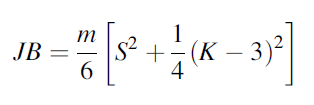
\includegraphics[width=0.7\linewidth]{MSQCChap4JBteststatistic}
\caption{}
\label{fig:MSQCChap4JBteststatistic}
\end{figure}
\end{frame}
%=============================================%
\begin{frame}[fragile]
where m is the sample size and S and K the skewness and kurtosis respectively.
The JB statistics follows a $\chi^2$ distribution with two degrees of freedom.
For more details see Jarque and Bera (1980), Jarque and Bera (1987), or Jarque
(2010).
Jarque (2010) offers the significance points table although statistical software
usually computes the p-values as:
p-value=1 - pchisq(STATISTIC, df = 2) or p-value = 1 – w2
JB,2
\end{frame}
%=============================================%
\begin{frame}[fragile]
At least three R packages include this test. They are: tseries, moments, and lawstat. In this context we use the first one:
> library("tseries")
Example 4.4
Using the \texttt{jarque.bera.test} function for each quality characteristics from the

bimetal1 dataset:

\end{frame}
%=============================================%
\begin{frame}[fragile]
Jarque-Bera Test
data: bimetal1[, 1]
X-squared = 0.22,
df = 2, p-value = 0.90
Jarque-Bera Test
data: bimetal1[, 3]
X-squared = 1.87,
df = 2, p-value = 0.39
Jarque-Bera Test
data: bimetal1
[, 5]
X-squared = 0.57,
df = 2, p-value = 0.75
Jarque Bera Test
data: bimetal1[, 2]
X-squared = 1.74, df = 2,
p-value = 0.42
Jarque Bera Test
data: bimetal1[, 4]
X-squared = 0.96, df = 2,
p-value = 0.62
\end{frame}
%=============================================%
\begin{frame}[fragile]
Notice that according to the p-values the normality assumption cannot be
rejected at alpha level = 0.05 or 0.10.
4.1 Tools of Support to MSQC 93
%-------------------------------------------------------------------------------------%
\end{frame}
\section{4.1.2.4 The Shapiro and Wilk (1965) Test}
\begin{frame}
The Shapiro and Wilk (1965) Test has become one of the most popular tests due to
its high performance.
The null hypothesis H0 is the sample that proceeds from a normal distribution
and possesses the statistics

%%Royston (1982) proposed the transformation ofWfor 7m2000 to normality
%%as follows:
%%x = ð1 - WÞl (4.22)
%%94 4 Tools of Support to MSQC
%-------------------------------------------------------------------------------------%

%and
%z = x - mx
%ð Þ
%sx
%(4.23)
R includes the built-in function \texttt{shapiro.test()} to compute this test.
\end{frame}
\subsection{Example 4.5}
\begin{frame}
The example below illustrates its use over the bimetal1 dataset. Using this function
individually for every quality characteristic
\begin{figure}
\centering
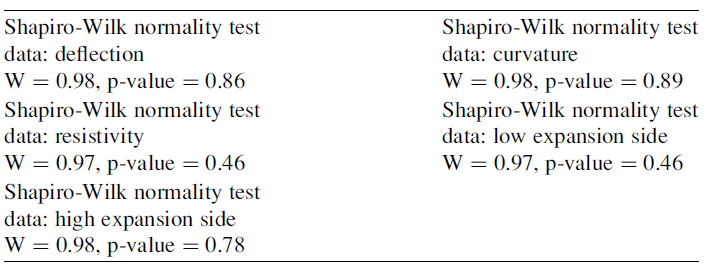
\includegraphics[width=0.7\linewidth]{MSQCChap4-ShapiroTest}
\caption{}
\label{fig:MSQCChap4-ShapiroTest}
\end{figure}

\end{frame}
\begin{frame}
On the other hand, Thode (2010) offers an excellent presentation of the most
powerful test and suggests a test based on moments like Shapiro-Wilks, Anderson-
Darling, and Jarque Bera. 
%% For more details see Thode (2002).

\end{frame}
%=============================================%

%---------------------------------------------------------------------%
\subsection{4.1.3 Assessing Multivariate Normality}
\begin{frame}[fragile]
	
Though the literature reflects that the proposals to test multivariate normality
exceed the 50 methods (see e.g.: (Mecklin and Mundfrom 2004)) these tools are
rarely applied in MSPC publications. This is due to the fact that as a general rule
these methods lack of simplicity and the software availability is limited.
Three of the most powerful tests are introduced in this section.

\end{frame}

%---------------------------------------------------------------------%
\section{4.1.3.1 Mardia (1970) Skewness and Kurtosis Test}

\begin{frame}
\frametitle{Mardia Test}
\large
The Mardia (1970) test is a generalization of the univariate skewness and kurtosis
test and becomes one of the most popular ones on assessment of multivariate
normality. The multivariate skewness and kurtosis are given by:
\begin{figure}
\centering
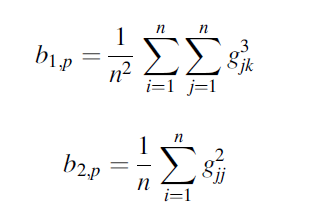
\includegraphics[width=0.7\linewidth]{MSQCChap4-MardiaTestStatistics}
\caption{}
\label{fig:MSQCChap4-MardiaTestStatistics}
\end{figure}
\end{frame}

%% 4.1 Tools of Support to MSQC 95
%-------------------------------------------------------------------------------------%

%---------------------------------------------------------------------%
%%1 where:
%%g3
%%jk
%%= xj - x
%% 0S-1ðxk - xÞ
%% 3
%%(4.26)
%%and
%%g2
%%jj
%%= xj - x
%% 0S-1 xj - x
%%  2
%%(4.27)
\begin{frame}
\frametitle{Mardia Test}
\large	
%----------------------------------%
Mardia (1970, 1974) provides the percentiles for b1,p and b2,p for many values of
p (quality characteristics) and many numbers of samples (m).
Mardia also proposed for b1,p an approximation to the $\chi^2$ distribution as follows:
%b1;p
%ðp þ 1Þðm þ 1Þðm þ 3Þ
%6 m þ 1 ð Þ p þ 1 ð Þ-6 ½ 
% w2a
%;½pðpþ1Þðpþ2Þ=6 (4.28)
%while for b2,p a normal approximation, being:
%b2;p  Nðpðp þ 2Þ; 8pðp þ 2Þ=mÞ (4.29)

The Mardia test is available from QRMlib and dprep R packages.

\end{frame}
\begin{frame}[fragile]
	\frametitle{Mardia Test}
	\large
Example 4.6

Then, to illustrate the Mardia Test return to the bimetal1 dataset.
Using the QRMlib package:
\begin{verbatim}
> MardiaTest(bimetal1)
# The R returns
$skewness
[1] 6.982112
$p.value
[1] 0.585327
$kurtosis
[1] 33.77373
$p.value
[1] 0.3490892
\end{verbatim}
%----------------------------------%
Regarding the p-value for skewness and kurtosis, there is no evidence of
departures from normality.
\end{frame}
\subsection{4.1.3.2 Henze and Zirkler (1990) Test}
\begin{frame}
	\frametitle{Henze and Zirkler}
	\large
Henze and Zirkler (1990) proposed a multivariate normality test based on the
empirical characteristic function. A wide number of simulation studies point out
the high performance of this test. See e.g.: (Thode 2002)

The statistics is given by:
\end{frame}
%% - 96 4 Tools of Support to MSQC
%-------------------------------------------------------------------%
%-------------------------------------------------------------------%
\subsection{Example 4.7}
\begin{frame}[fragile]
\frametitle{Henze and Zirkler}
\large
The following example shows the application of the test using also the bimetal1
data:
\begin{verbatim}
> HZ.test(bimetal1)
p-value HZ statistic
[1] 0.61 0.77
\end{verbatim}
According to the results obtained, p-value = 0.77, which is a high value; there is
no evidence to reject the assumption of multivariate normality.
\end{frame}
\subsection{4.1.3.3 Royston (1992)Test}
\begin{frame}
	\frametitle{Royston Test}
Another powerful test was proposed by Royston (1983) which is a multivariate extension
of the Shapiro andWilks normality test (see Royston 1982, 1983, 1992, 1995).
The statistic recommended by Royston is
[Royston TS]

There are two ways to compute Zj according to the number of  observations:


(4.41)
Wj is the statistics of the univariate Shapiro-Wilks test. (See the previous
section.)
\end{frame}
%--------------------------------------%
%% where
%% g = -2:273 þ 0:459n (4.42)
%% m = 0:544 - 0:39978n þ 0:025054n2 - 0:0006714n3 (4.43)
%% s = exp 1:3822 - 0:77875n þ 0:062767n2 - 0:0020322n3 
%% (4.44)
% and for 12 < = x < = 2000

%% 98 4 Tools of Support to MSQC
%-------------------------------------------------------------------------------------%

\section{4.1.4 Solutions to Departures from Normality}
\begin{frame}
\frametitle{Departures from Normality}
\Large
\begin{itemize}
	\item Practically, it is common to get variables with non-normal distribution and one
	alternative is to transform the data. 
	\item The transformation of the data is the application
	of a mathematical function to the original dataset.
	\item In a multivariate context this solution could be addressed to a marginal or
	multivariate approach. 
	\item In this section two marginal solutions and one multivariate
	are introduced.
\end{itemize}
\end{frame}
%================================================%
\begin{frame}
\begin{itemize}
	\item There are many simple transformations used in practice: $\sqrt{x}$, log(x), arcsin($\sqrt{x}$),
	etc (see, e.g., (Juran and Godfrey 1998) Sect. 4.4)
	\item Another is the well-known Box-Cox Transformation (BCT) that is probably the
	most used one for practitioners and professionals of quality control. 
	\item Finally, another
	type of transformation (although not so well known) is the Johnson’s system of
	distributions recognized as the \textbf{\textit{Johnson Transformation (JT)}}.
\end{itemize}

\end{frame}
%----------------------------------------------------------------------------%
\subsection{4.1.4.1 Box-Cox Transformation (BCT)}
\begin{frame}
The family of Box-Cox is a power transformation suggested by Box and Cox
(1964). It is given by:
%yi =
%xli
%- 1
%l
%for l 6= 0
%log xi ð Þ for l = 0
%8<
%: (4.52)
where xi is the original dataset, l (lambda) is the power and yi the new observations.
\end{frame}
%=====================================%
\begin{frame}
\begin{itemize}
	\item One alternative, in order to find the optimal value of l, is using the value that maximizes the logarithm of the likelihood function. 
%	\item For more details see Box and Cox (1964) or Venables and Ripley (2002).
	
	\item The BCT is widely used to improve the normality in some practical situations and a lot of statistical packages provide this application. 
	\item An advantage is the easy algorithm to transform the data while a disadvantage is that it does not allow
	negative data values, though it can be solved by adding a constant to the original dataset.
	
	\item There are many functions in \texttt{R} that perform the BCT transformation but we will use the \texttt{powerTransform} included in \texttt{car} package.
\end{itemize}

\end{frame}
%----------------------------------------------------------------------------%
\subsection{4.1.4.2 Johnson Transformation (JT)}
\begin{frame}
The Z family of distributions was presented in Johnson (1949) and is composed by
three distributions named \textbf{\textit{Unbounded (SU)}}, \textbf{\textit{Lognormal (SL)}}, and \textbf{\textit{Bounded (SB)}}
which allow to transform into a normal distribution through selecting one of the three of them. The transformations are:

\end{frame}
%% 100 4 Tools of Support to MSQC
%-------------------------------------------------------------------------------------%



\subsubsection{Example 4.10}
\begin{frame}[fragile]
Coming back to the bimetal1 dataset, the marginal independence could be assessed.
\begin{verbatim}
> par(mfrow = c(3,2))
> for( i in 1 : ncol(bimetal1) ){
> par(mar = c(4.1,4.5,1,1))
> acf(bimetal1[,i],lag = 7,las = 1)}
\end{verbatim}
\end{frame}
%-------------------------------------------------%
\begin{frame}
Notice that when lag = 0 the correlation is 1. This can be proved easily in formula x.
There is no evidence of relation between adjacent observations; that is, there is marginal randomness.
This tool can be complemented with the use of another such as: Box-Pierce, Ljung-Box or Runs Test (Fig. 4.5).

\end{frame}

%%PAGE 105
\begin{frame}
When time dependence is detected the problem should be addressed in two different ways: by using a specific control chart such as the proposal by Apley and Tsung (2002) and Kalagonda and Kulkarni (2004) or by modifying the data removing the autocorrelation effects. About the latter point a possible solution is to decompose it in multivariate autoregressive model and analyze the resultant
residuals which should present independency and MVN (Mason and Young 2001).
\end{frame}

\end{document}